\documentclass[11pt,a4paper]{article}
\usepackage[utf8]{inputenc}\usepackage[T1]{fontenc}\usepackage[brazilian]{babel}
\usepackage{graphicx,booktabs,float,hyperref,geometry}\geometry{margin=2.2cm}
\graphicspath{{../reports/figures/}}
\begin{document}
\begin{titlepage}\centering
{\large UNIVERSIDADE FEDERAL DO RIO GRANDE DO NORTE\\DCT1401 -- Inteligência Artificial\\}\vspace{2cm}
{\LARGE\bfseries Avaliação Comparativa de Modelos:\\Sistema Especialista, Árvore de Decisão e Ensemble Learning\par}
\vspace{2cm}Aluno: Jonas Jeronimo Cirilo Silva \quad Matrícula: 20240026090\\[1ex]
Dataset: \url{https://www.kaggle.com/datasets/mobeenfatimah/human-digital-twin-dataset-for-ai-and-healthcare}\\[1ex]
Repositório: \url{https://github.com/xonazz/IA\_thomas2}
\end{titlepage}

\section{Introdução}
Este relatório compara três famílias de modelos --- sistema especialista (regras SE-ENTÃO), árvore de decisão e ensembles
(Random Forest e Gradient Boosting) --- em dois problemas sobre o conjunto \emph{Human Digital Twin} (Kaggle), usando o arquivo
\texttt{digital\_twin\_profile.csv}: 5000 indivíduos sintéticos e 30 colunas (demografia, hábitos, sinais vitais e diagnósticos).
O conjunto é sintético, o que explica parte dos resultados discutidos adiante. Há 150 valores ausentes em cada uma de cinco colunas
(\texttt{BMI}, \texttt{Heart\_Rate}, \texttt{Physical\_Activity}, \texttt{Daily\_Water\_Intake\_L}, \texttt{Sleep\_Hours}), tratados por imputação dentro do \texttt{Pipeline}.
\textbf{Classificação:} prever \texttt{Hypertension} (Yes/No; 17,2\% de \emph{Yes}), com 24 features e \emph{sem} as colunas de pressão arterial
e sem diagnósticos, pois a pressão define a hipertensão e tornaria o problema trivial.
\textbf{Regressão:} prever \texttt{Blood\_Pressure\_Systolic} (mmHg), com 26 features: as mesmas, mais os diagnósticos
\texttt{Hypertension} e \texttt{Diabetes} (variáveis registradas à parte) e sem a pressão diastólica. Sem os diagnósticos, a regressão não tem
sinal algum (R$^2$ de validação cruzada negativo em teste preliminar). \textbf{TODO (aluno):} se os targets da atividade anterior forem outros, justificar aqui a mudança.

\section{Protocolo Experimental}
Divisão 80/20 com \texttt{random\_state=42} (estratificada na classificação), a mesma para os três tipos de modelo: 4000 amostras de treino e 1000 de teste
(classificação: 688 e 172 casos \emph{Yes} no treino e no teste). O teste só foi usado na avaliação final; os
hiperparâmetros foram ajustados por validação cruzada de 5 folds no treino (\texttt{GridSearchCV} para a árvore e
\texttt{RandomizedSearchCV} para os ensembles; métrica de seleção: F1 macro e RMSE). Imputação e codificação ficam em um
\texttt{Pipeline} ajustado só no treino. Um \emph{baseline} constante (classe majoritária / média) serve de referência.
Ambiente de execução dos experimentos reportados: Linux-6.18.44-fc-v153-x86\_64-with-glibc2.39, Python 3.13.17, 2 núcleo(s), 7.8 GB RAM.
\textbf{TODO (aluno):} reexecutar \texttt{python run\_all.py} na sua máquina e substituir pelo seu hardware. Energia estimada como potência
média assumida (45 W) $\times$ tempo, convertida com 45,8 gCO$_2$/kWh (fator do Brasil, Aula 08); o \texttt{codecarbon} não foi utilizado.

\section{Sistema Especialista}
A base de conhecimento fica em arquivo texto, separada do motor de inferência (encadeamento para frente, com resolução de
conflito por prioridade e regra padrão final). Cada regra usa só conjunções (E). Os limiares foram definidos observando apenas o treino
(taxas de hipertensão por faixa de IMC e idade) e conhecimento de domínio. Base de classificação (6 regras; tipos: relação, heurística, diretriz e estratégia):
\begin{verbatim}
R1 | relação | prio=1 | SE BMI >= 30 E Age >= 60 ENTÃO Yes
R2 | relação | prio=2 | SE BMI >= 30 E Age >= 45 ENTÃO Yes
R3 | relação | prio=3 | SE BMI >= 27.5 E Age >= 60 ENTÃO Yes
R4 | heurística | prio=4 | SE BMI >= 27.5 E Age >= 45 E Family_History == Yes ENTÃO Yes
R5 | diretriz | prio=5 | SE BMI < 25 ENTÃO No
R6 | estratégia | prio=6 | SE VERDADEIRO ENTÃO No
\end{verbatim}
Base de regressão (5 regras; o consequente é a média da pressão sistólica no treino de cada combinação de diagnósticos):
\begin{verbatim}
R1 | relação | prio=1 | SE Hypertension == Yes E Diabetes == No ENTÃO PA = 138.76
R2 | relação | prio=2 | SE Hypertension == Yes E Diabetes == Yes ENTÃO PA = 137.03
R3 | relação | prio=3 | SE Hypertension == No E Diabetes == No ENTÃO PA = 121.34
R4 | relação | prio=4 | SE Hypertension == No E Diabetes == Yes ENTÃO PA = 120.97
R5 | estratégia | prio=5 | SE VERDADEIRO ENTÃO PA = 124.19
\end{verbatim}
O sistema especialista não produz probabilidades; para as curvas ROC e PR usou-se a distribuição de classes das amostras de treino em que
cada regra disparou (suavização de Laplace). É uma pontuação em degraus (seis valores distintos), o que limita as curvas.
\paragraph{Cronometragem.} \textbf{TODO (aluno):} inserir a tabela de cronometragem (\texttt{logs/cronometro\_regras.csv}): no mínimo 3 sessões por problema, com data, horário, interrupções, nº de regras, tempo total, média, desvio-padrão e tempo médio por regra. Rode \texttt{python -m src.cronometro} e depois \texttt{python -m src.make\_report}.

\section{Árvore de Decisão}
Comparou-se Gini e entropia (classificação) e erro quadrático e erro absoluto (regressão), junto com \texttt{max\_depth},
\texttt{min\_samples\_leaf}, \texttt{ccp\_alpha} e (na classificação) \texttt{class\_weight}. Na classificação os dois critérios empataram na validação cruzada
(F1 macro 0,7031 e 0,7031); na regressão o erro quadrático foi um pouco melhor (RMSE 13,767 contra 13,789).
Melhor árvore de classificação: entropia, \texttt{max\_depth=3, min\_samples\_leaf=1, ccp\_alpha=0,005}
(profundidade efetiva 2, 5 nós, 3 folhas). Melhor árvore de regressão: erro quadrático,
profundidade 3, 15 nós, 8 folhas.
As árvores sem restrição acertam 100\% do treino, mas o F1 macro no teste cai para 0,58 (gini) e 0,55 (entropia), pior que a árvore ajustada (0,68), e na regressão o R$^2$ no teste é negativo (-0,64): overfitting evidente.
\begin{figure}[H]\centering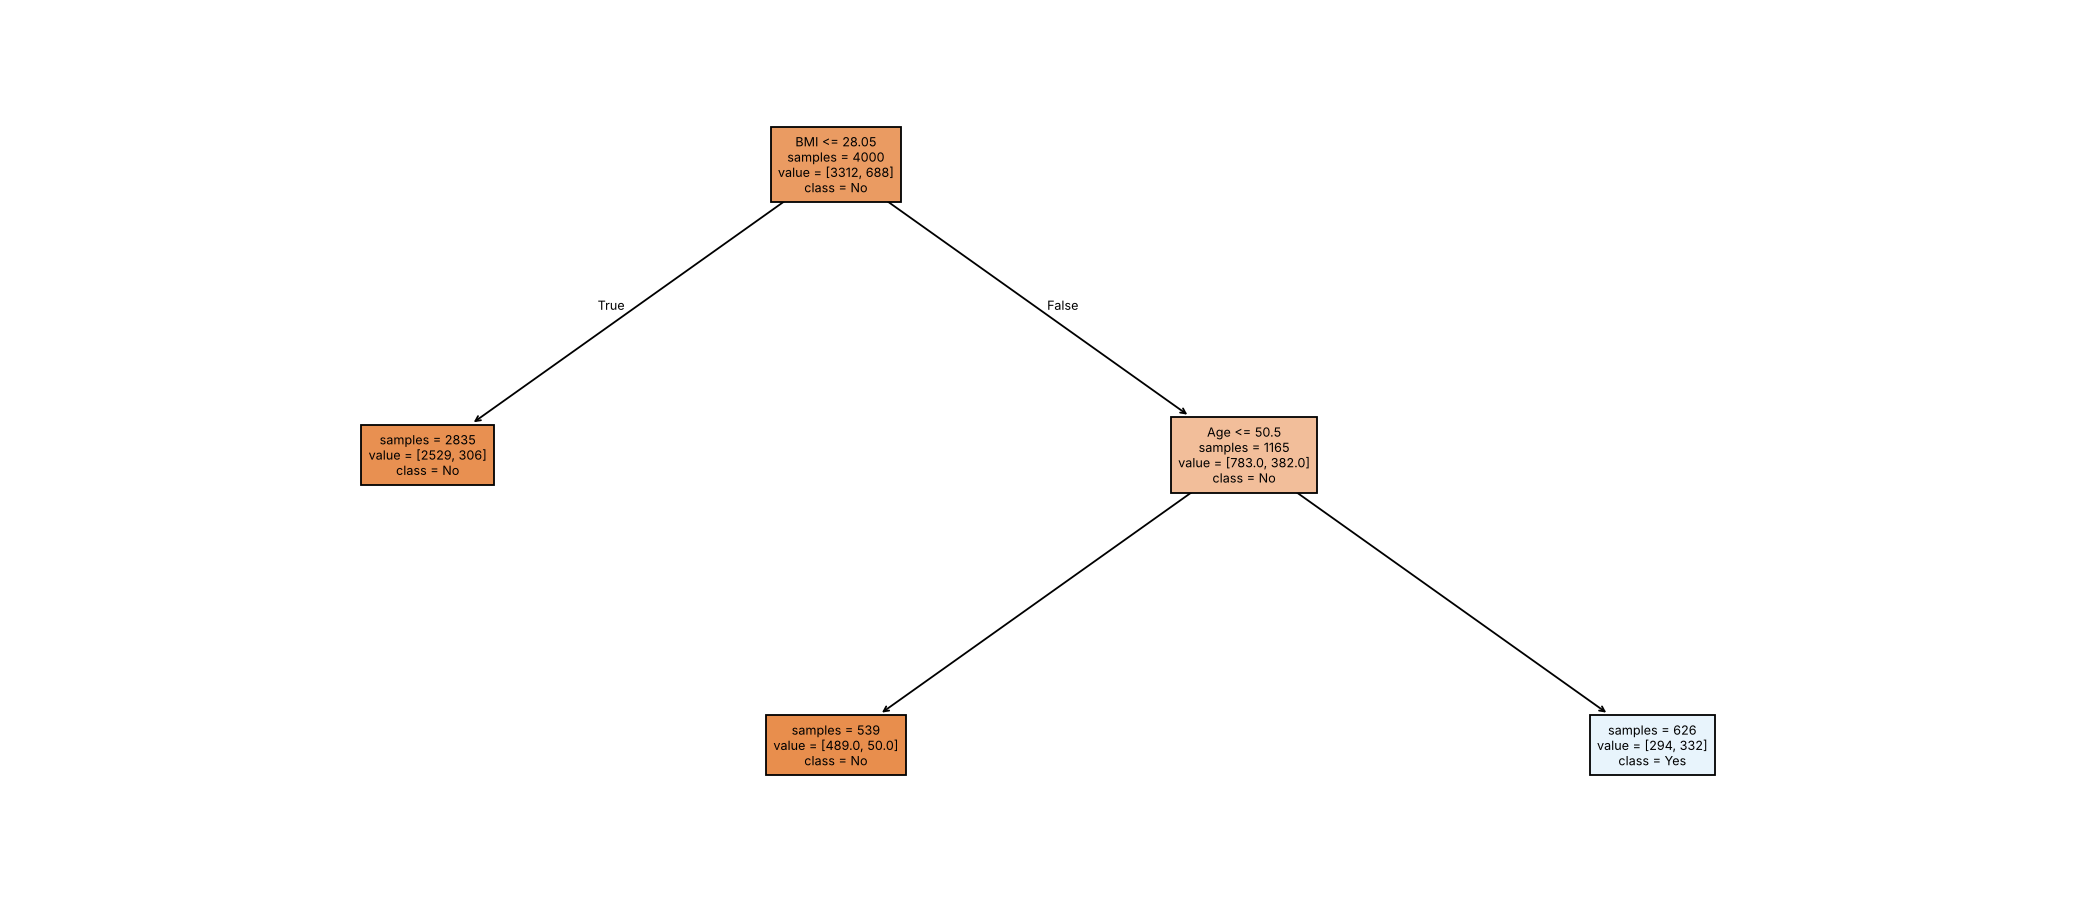
\includegraphics[width=\textwidth]{arvore_clf.png}\caption{Árvore ajustada (classificação).}\end{figure}
\paragraph{Três regras extraídas da árvore de classificação e comparação com o especialista.} A árvore tem exatamente três folhas:
\begin{enumerate}
\item IMC $\le$ 28,05 $\Rightarrow$ No. Corresponde à regra R5 do especialista (IMC $<$ 25 $\Rightarrow$ No) e à regra padrão R6, com um limiar de IMC mais alto aprendido dos dados.
\item IMC $>$ 28,05 e idade $\le$ 50,5 $\Rightarrow$ No. O especialista não tem regra equivalente: suas regras R2 e R4 já preveem \emph{Yes} a partir de 45 anos, ou seja, a árvore é mais conservadora para quem tem 45 a 50 anos.
\item IMC $>$ 28,05 e idade $>$ 50,5 $\Rightarrow$ Yes. Resume as regras R1 a R3 do especialista (IMC $\ge$ 27,5 ou 30 com idade $\ge$ 45 ou 60) em uma só.
\end{enumerate}
O padrão é o mesmo: IMC e idade carregam o sinal. A árvore aprende limiares únicos e mais simples; o especialista tem mais regras, mas depende de quem as escreve.
Na regressão, a árvore usa \texttt{Hypertension} na raiz; os demais cortes (tempo de tela, altura, frequência cardíaca) são ruído.

\section{Ensemble Learning}
Random Forest e Gradient Boosting, ajustados por busca aleatória (\texttt{n\_estimators}, \texttt{max\_depth}, \texttt{max\_features},
\texttt{min\_samples\_leaf}, \texttt{learning\_rate}, \texttt{subsample}). Classificação: RF com 100 árvores, profundidade 16, max\_features=0,5, class\_weight=balanced;
GB com 100 estimadores, profundidade 4, taxa 0,1, subsample=0,7.
Regressão: RF com 200 árvores e profundidade 10; GB com 100 estimadores, profundidade 2 e taxa 0,05.
\paragraph{Erro $\times$ número de árvores (Random Forest).} Na classificação, o erro de validação cruzada (1 $-$ F1 macro) cai de 0,434 com 1 árvore para 0,324 com 10, 0,307 com 50 e 0,303 com 200, enquanto o erro de treino fica em torno de 0,10.
Na regressão o RMSE de validação vai de 15,57 para 13,83 (50 árvores) e 13,79 (200 árvores).
A média de muitas árvores reduz a variância da árvore isolada; depois de $\sim$50 árvores o ganho é desprezível. A distância entre erro de treino e de validação, que não fecha, mostra que a floresta ainda memoriza parte do ruído (variância residual), e que o erro restante é sobretudo ruído irredutível.
\begin{figure}[H]\centering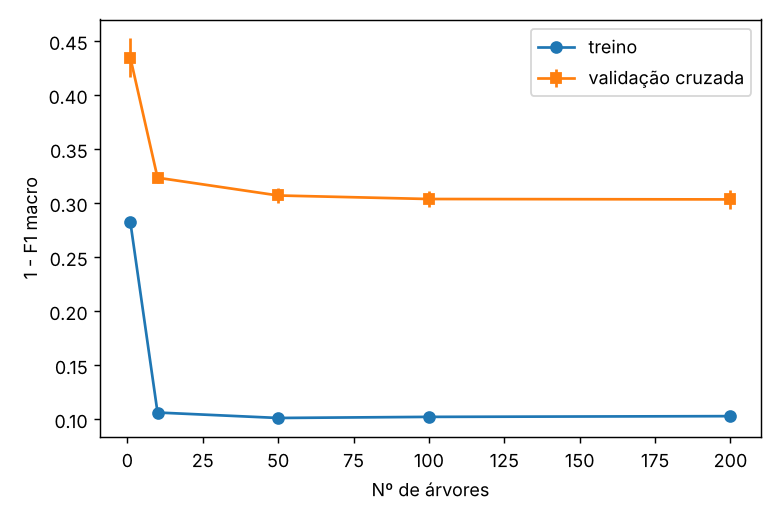
\includegraphics[width=.48\textwidth]{rf_curva_clf.png}
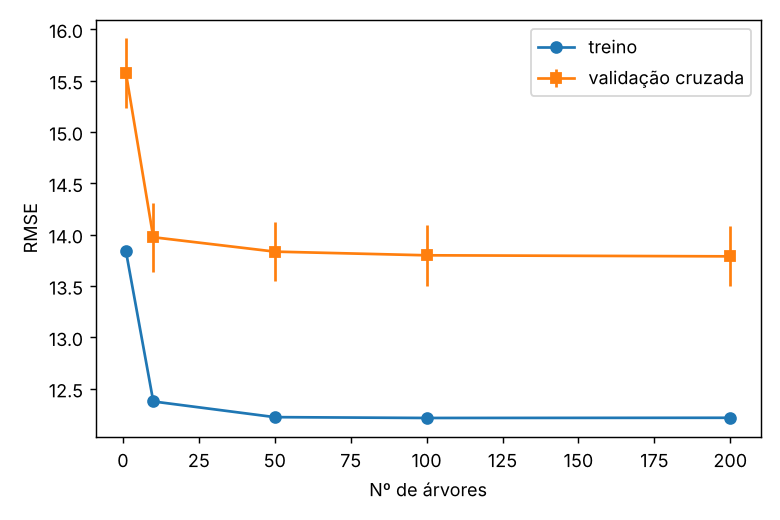
\includegraphics[width=.48\textwidth]{rf_curva_reg.png}\caption{Erro $\times$ número de árvores (RF).}\end{figure}
\paragraph{Importância das features.} Na classificação, a árvore usa apenas idade (0,52) e IMC (0,48); na RF e no GB, IMC e idade também lideram
(RF: 0,16 e 0,15), com o resto da importância diluída em variáveis sem relação real (peso, altura, renda, tempo de tela). São as variáveis das regras R1 a R5 do especialista.
Na regressão, \texttt{Hypertension} concentra a importância (árvore: 0,94; GB: 0,88; RF: 0,43), e o especialista usa exatamente essa variável (mais \texttt{Diabetes}, que quase não pesa).
\begin{figure}[H]\centering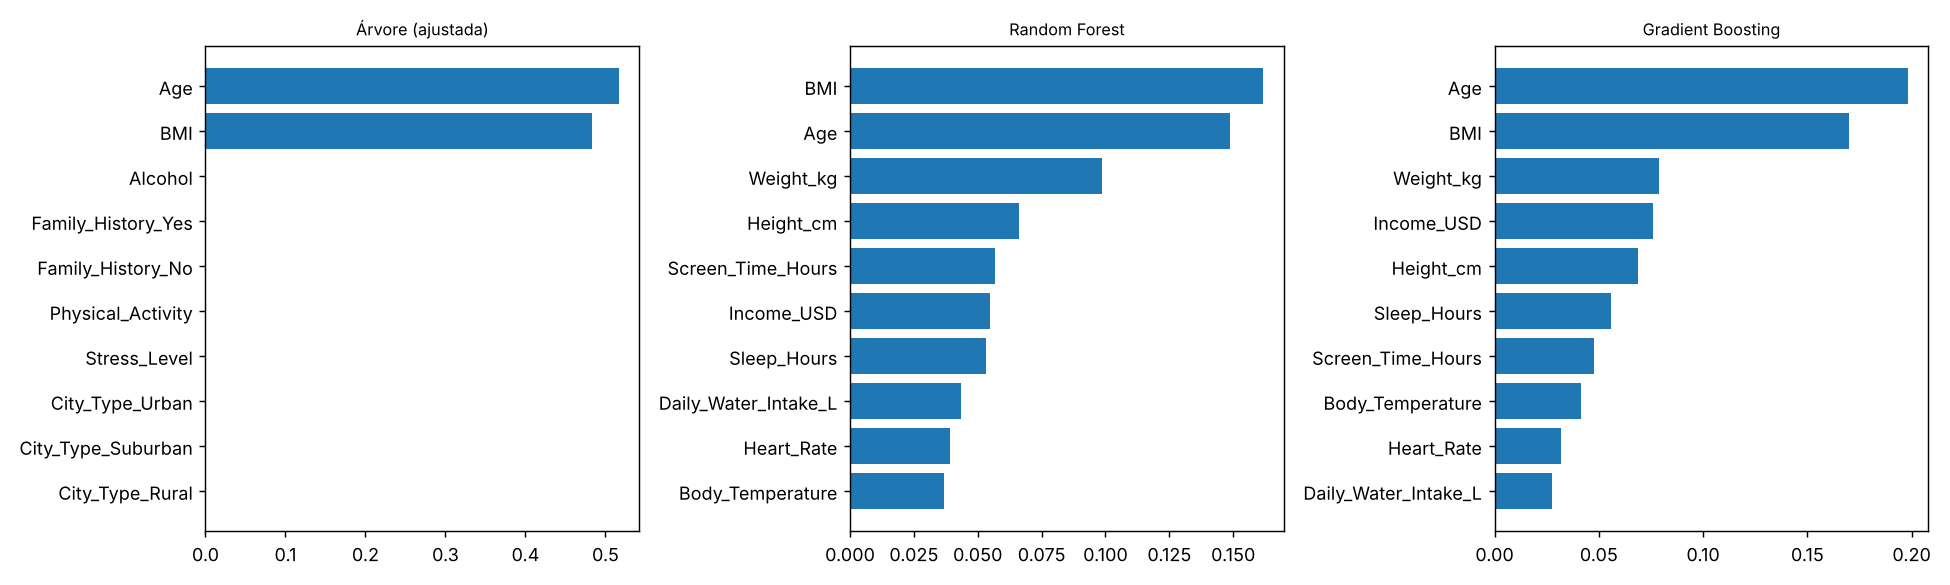
\includegraphics[width=.48\textwidth]{importancias_clf.png}
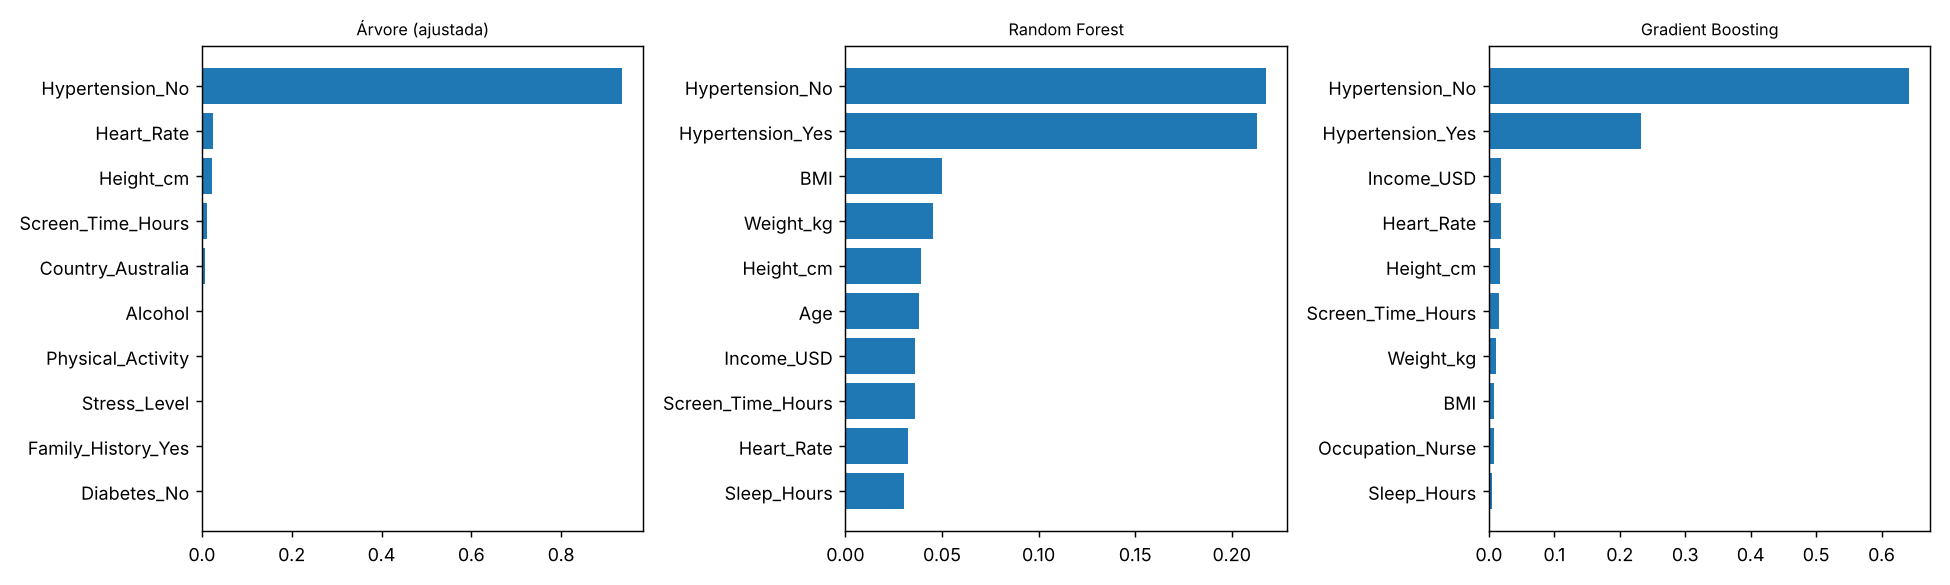
\includegraphics[width=.48\textwidth]{importancias_reg.png}\caption{Importância das features (impureza).}\end{figure}

\section{Resultados}
\begin{table}[H]\centering\scriptsize\resizebox{\ifdim\width>\linewidth\linewidth\else\width\fi}{!}{%
\begin{tabular}{lrrrrrrrrrr}\toprule
modelo & Accuracy & Precision\_macro & Recall\_macro & F1\_macro & F1\_weighted & Precision\_pos & Recall\_pos & F1\_pos & ROC\_AUC & PR\_AUC \\\midrule
Baseline (constante) & 0,828 & 0,414 & 0,500 & 0,453 & 0,750 & 0,000 & 0,000 & 0,000 & 0,500 & 0,172 \\
Sist. Especialista & 0,802 & 0,657 & 0,664 & 0,660 & 0,804 & 0,429 & 0,453 & 0,441 & 0,675 & 0,305 \\
Árvore sem poda (gini) & 0,746 & 0,577 & 0,586 & 0,581 & 0,753 & 0,295 & 0,343 & 0,317 & 0,586 & 0,214 \\
Árvore sem poda (entropy) & 0,728 & 0,549 & 0,555 & 0,551 & 0,736 & 0,250 & 0,291 & 0,269 & 0,555 & 0,195 \\
Árvore (ajustada) & 0,825 & 0,689 & 0,676 & 0,682 & 0,822 & 0,490 & 0,448 & 0,468 & 0,674 & 0,318 \\
Random Forest & 0,824 & 0,688 & 0,677 & 0,682 & 0,821 & 0,487 & 0,453 & 0,470 & 0,682 & 0,370 \\
Gradient Boosting & 0,830 & 0,684 & 0,589 & 0,606 & 0,801 & 0,514 & 0,221 & 0,309 & 0,685 & 0,387 \\
\bottomrule\end{tabular}}
\caption{Classificação (Hypertension): métricas no conjunto de teste.}\label{tab:met_clf}\end{table}

\begin{table}[H]\centering\scriptsize\resizebox{\ifdim\width>\linewidth\linewidth\else\width\fi}{!}{%
\begin{tabular}{lrrrrr}\toprule
modelo & F1\_macro\_treino & F1\_macro\_teste & gap & gap\_relativo & diagnostico \\\midrule
Baseline (constante) & 0,453 & 0,453 & 0,000 & 0,000 & underfitting \\
Sist. Especialista & 0,679 & 0,660 & 0,019 & 0,028 & bem ajustado \\
Árvore sem poda (gini) & 1,000 & 0,581 & 0,419 & 0,419 & overfitting \\
Árvore sem poda (entropy) & 1,000 & 0,551 & 0,449 & 0,449 & overfitting \\
Árvore (ajustada) & 0,704 & 0,682 & 0,022 & 0,032 & bem ajustado \\
Random Forest & 0,898 & 0,682 & 0,216 & 0,240 & overfitting \\
Gradient Boosting & 0,808 & 0,606 & 0,202 & 0,250 & overfitting \\
\bottomrule\end{tabular}}
\caption{Classificação: gap de generalização (F1 macro treino $-$ teste).}\label{tab:gap_clf}\end{table}

\begin{table}[H]\centering\scriptsize\resizebox{\ifdim\width>\linewidth\linewidth\else\width\fi}{!}{%
\begin{tabular}{lrr}\toprule
modelo & F1\_macro\_cv\_media & F1\_macro\_cv\_desvio \\\midrule
Árvore (ajustada) & 0,7031 & 0,0111 \\
Random Forest & 0,6961 & 0,0075 \\
Gradient Boosting & 0,6315 & 0,0143 \\
\bottomrule\end{tabular}}
\caption{Classificação: validação cruzada (5 folds, treino).}\label{tab:cv_clf}\end{table}

\begin{table}[H]\centering\scriptsize\resizebox{\ifdim\width>\linewidth\linewidth\else\width\fi}{!}{%
\begin{tabular}{lrrrrrr}\toprule
modelo & treino\_s & inf\_ms/amostra & vazao/s & pico\_inf\_kb & disco\_kb & CO2\_treino\_g \\\midrule
Sist. Especialista & -- & 0,04803 & 2,082e+04 & 294,3 & 0,5986 & -- \\
Árvore (ajustada) & 0,06612 & 0,0364 & 2,747e+04 & 1483 & 9,02 & 3,785e-05 \\
Random Forest & 1,664 & 0,07955 & 1,257e+04 & 1552 & 3703 & 0,0009525 \\
Gradient Boosting & 1,407 & 0,03789 & 2,639e+04 & 1548 & 252,2 & 0,0008054 \\
\bottomrule\end{tabular}}
\caption{Classificação: eficiência computacional (inferência no teste, 1000 amostras).}\label{tab:ef_clf}\end{table}

\begin{table}[H]\centering\scriptsize\resizebox{\ifdim\width>\linewidth\linewidth\else\width\fi}{!}{%
\begin{tabular}{lrrrrrr}\toprule
modelo & MAE & MSE & RMSE & MAPE\_\% & R2 & MedAE \\\midrule
Baseline (constante) & 12,472 & 237,966 & 15,426 & 10,169 & -0,003 & 10,812 \\
Sist. Especialista & 11,108 & 188,955 & 13,746 & 9,112 & 0,203 & 9,660 \\
Árvore sem poda (squared\_error) & 16,168 & 388,590 & 19,713 & 13,147 & -0,638 & 14,000 \\
Árvore sem poda (absolute\_error) & 16,093 & 394,873 & 19,871 & 13,123 & -0,665 & 14,000 \\
Árvore (ajustada) & 11,111 & 189,001 & 13,748 & 9,106 & 0,203 & 9,500 \\
Random Forest & 11,161 & 190,372 & 13,798 & 9,146 & 0,197 & 9,676 \\
Gradient Boosting & 11,095 & 188,756 & 13,739 & 9,094 & 0,204 & 9,444 \\
\bottomrule\end{tabular}}
\caption{Regressão (Blood\_Pressure\_Systolic): métricas no teste.}\label{tab:met_reg}\end{table}

\begin{table}[H]\centering\scriptsize\resizebox{\ifdim\width>\linewidth\linewidth\else\width\fi}{!}{%
\begin{tabular}{lrrrrr}\toprule
modelo & RMSE\_treino & RMSE\_teste & gap & gap\_relativo & diagnostico \\\midrule
Baseline (constante) & 15,16 & 15,43 & 0,2706 & 0,01786 & underfitting \\
Sist. Especialista & 13,73 & 13,75 & 0,01559 & 0,001136 & bem ajustado \\
Árvore sem poda (squared\_error) & 0 & 19,71 & 19,71 & -- & overfitting \\
Árvore sem poda (absolute\_error) & 0 & 19,87 & 19,87 & -- & overfitting \\
Árvore (ajustada) & 13,63 & 13,75 & 0,1154 & 0,008465 & bem ajustado \\
Random Forest & 12,22 & 13,8 & 1,582 & 0,1295 & overfitting \\
Gradient Boosting & 13,53 & 13,74 & 0,2138 & 0,01581 & bem ajustado \\
\bottomrule\end{tabular}}
\caption{Regressão: gap de generalização (RMSE teste $-$ treino).}\label{tab:gap_reg}\end{table}

\begin{table}[H]\centering\scriptsize\resizebox{\ifdim\width>\linewidth\linewidth\else\width\fi}{!}{%
\begin{tabular}{lrr}\toprule
modelo & RMSE\_cv\_media & RMSE\_cv\_desvio \\\midrule
Árvore (ajustada) & 13,7666 & 0,2653 \\
Random Forest & 13,7876 & 0,2924 \\
Gradient Boosting & 13,7556 & 0,2649 \\
\bottomrule\end{tabular}}
\caption{Regressão: validação cruzada (5 folds, treino).}\label{tab:cv_reg}\end{table}

\begin{table}[H]\centering\scriptsize\resizebox{\ifdim\width>\linewidth\linewidth\else\width\fi}{!}{%
\begin{tabular}{lrrrrrr}\toprule
modelo & treino\_s & inf\_ms/amostra & vazao/s & pico\_inf\_kb & disco\_kb & CO2\_treino\_g \\\midrule
Sist. Especialista & -- & 0,04252 & 2,352e+04 & 314,2 & 0,5938 & -- \\
Árvore (ajustada) & 0,05729 & 0,0387 & 2,584e+04 & 1574 & 9,887 & 3,28e-05 \\
Random Forest & 0,9844 & 0,137 & 7299 & 1681 & 4309 & 0,0005636 \\
Gradient Boosting & 0,9413 & 0,04247 & 2,355e+04 & 1611 & 90,39 & 0,0005389 \\
\bottomrule\end{tabular}}
\caption{Regressão: eficiência computacional.}\label{tab:ef_reg}\end{table}

\begin{figure}[H]\centering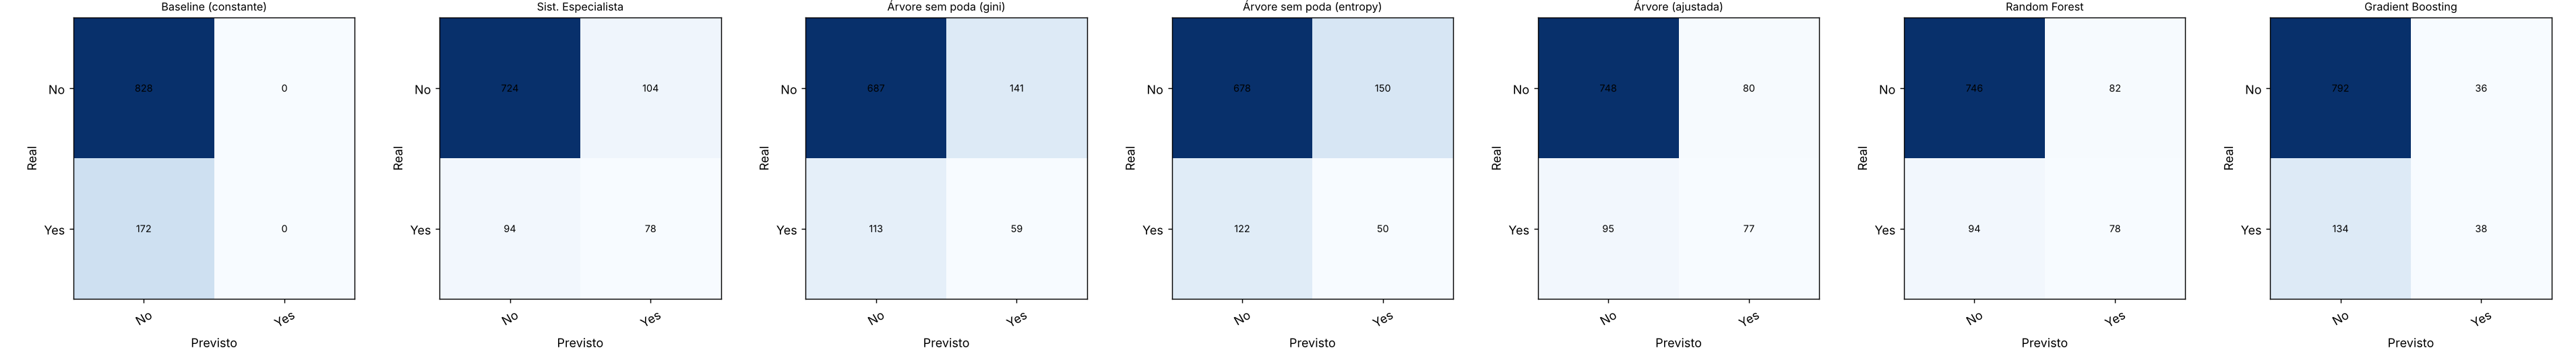
\includegraphics[width=\textwidth]{matrizes_confusao.png}\caption{Matrizes de confusão (teste, classificação).}\end{figure}
\begin{figure}[H]\centering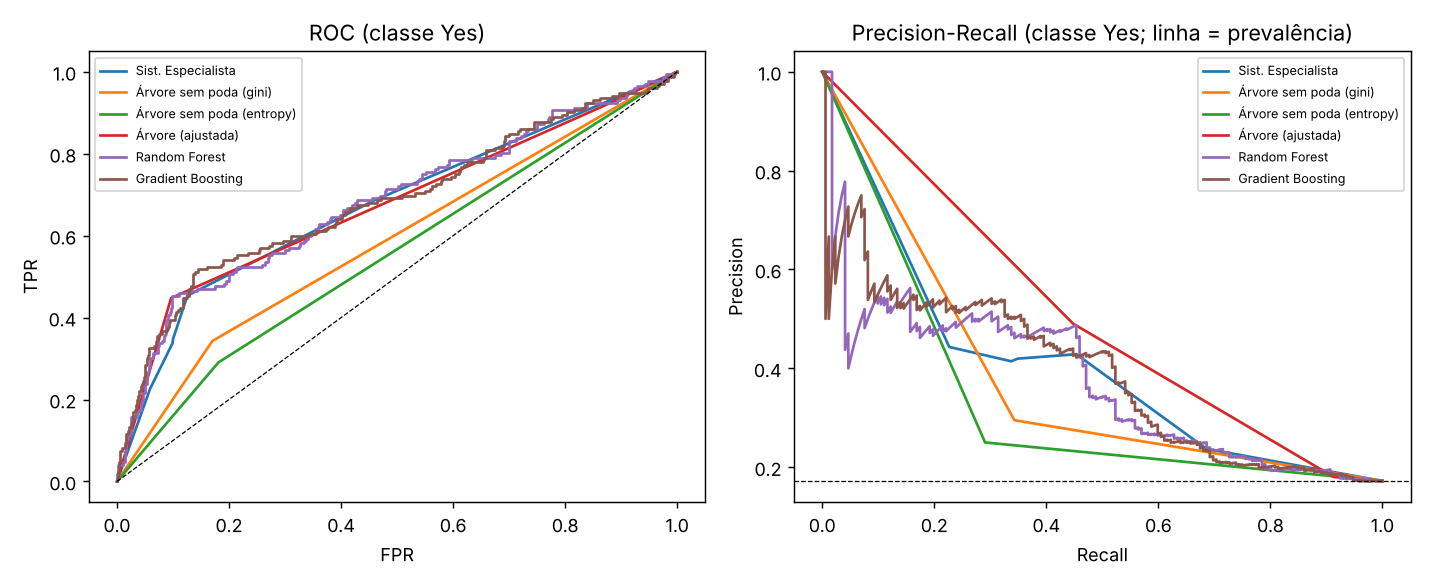
\includegraphics[width=\textwidth]{roc_pr.png}\caption{Curvas ROC e Precision-Recall da classe \emph{Yes} (teste).}\end{figure}
\begin{figure}[H]\centering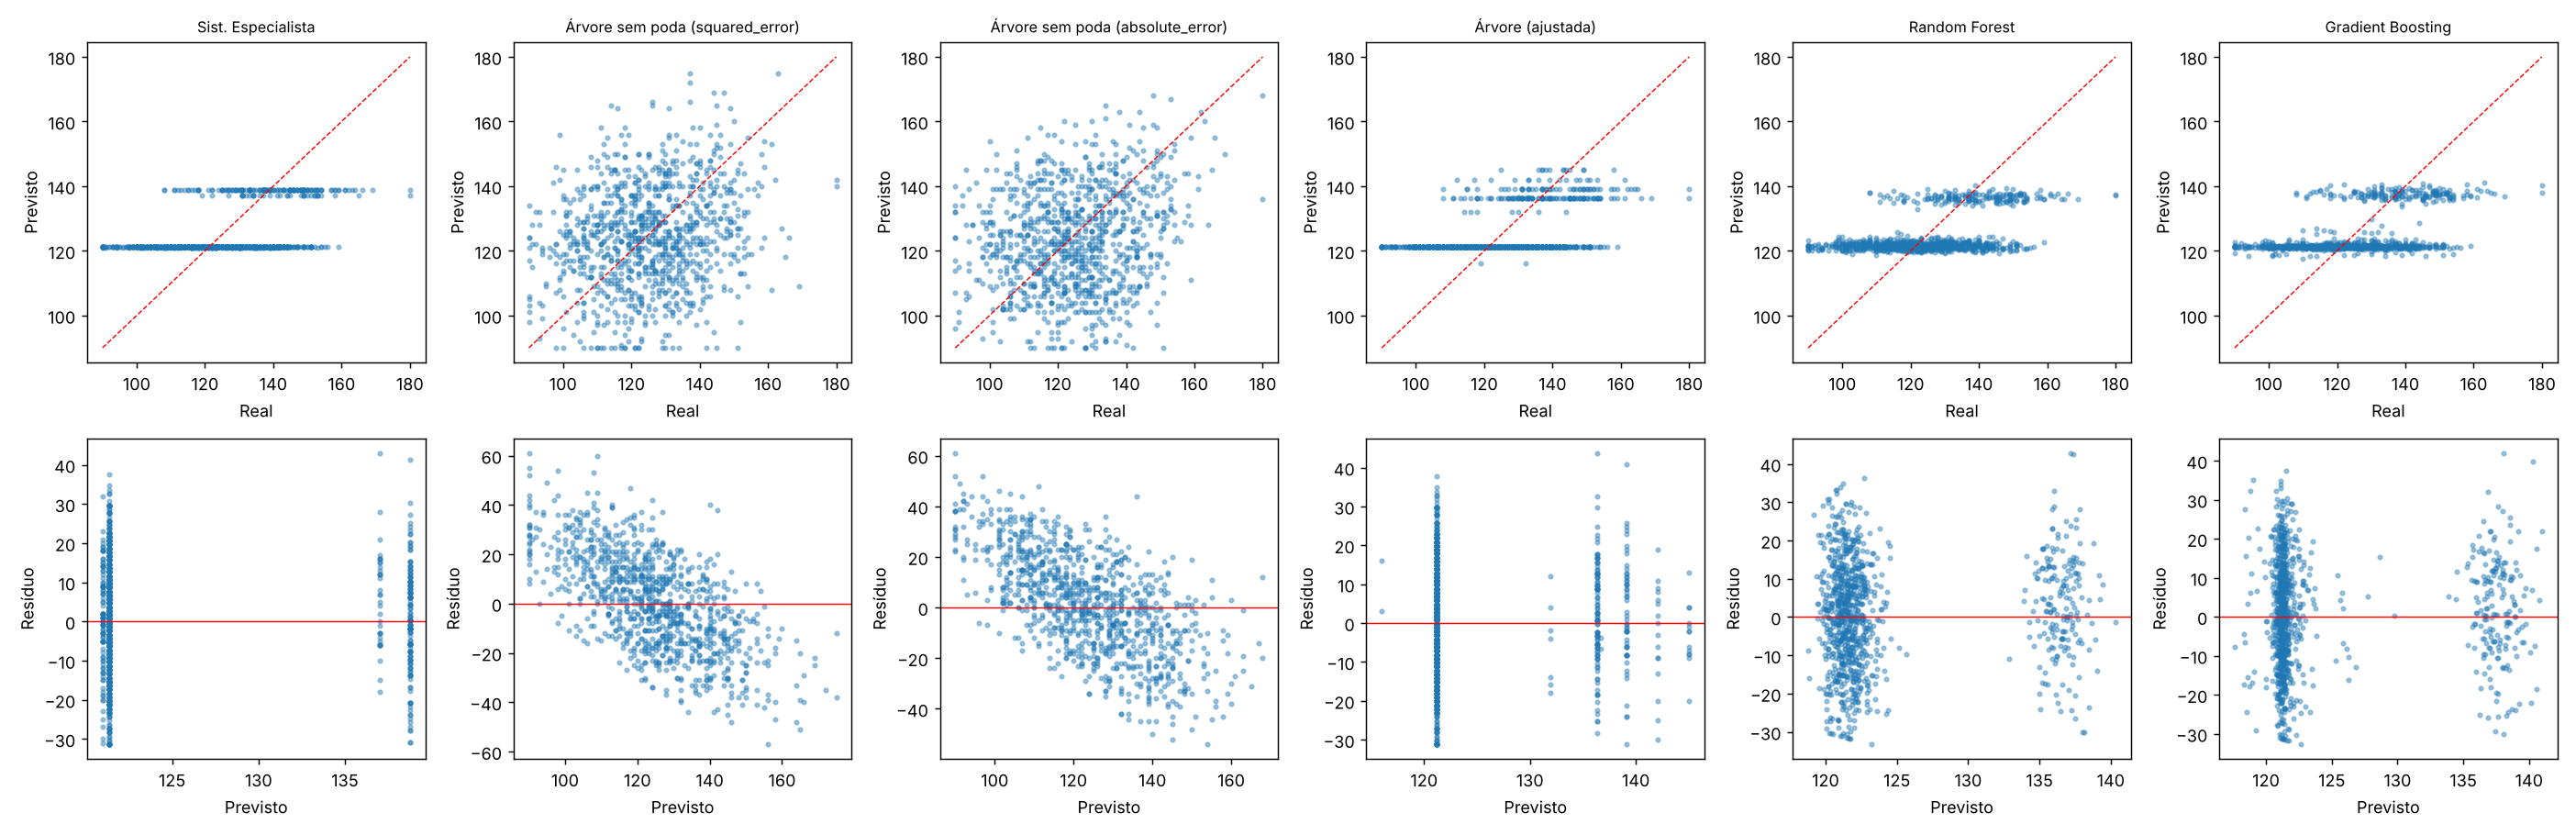
\includegraphics[width=\textwidth]{real_vs_previsto_residuos.png}\caption{Real vs.\ previsto e resíduos (regressão).}\end{figure}
\paragraph{Escolha das métricas.} Na classificação, a Accuracy engana: o baseline que sempre responde \emph{No} já tem Accuracy de 0,828, maior que a do especialista (0,802) e praticamente igual à da árvore ajustada, da RF e do GB, apesar de não acertar nenhum \emph{Yes}. Usou-se F1 macro como
métrica principal (baseline: 0,453), por dar o mesmo peso à classe rara; ROC-AUC e PR-AUC complementam (a PR-AUC do baseline é a prevalência, 0,172). Em triagem clínica, o falso negativo (hipertenso não detectado) é o erro mais custoso, por isso o recall da classe positiva também é reportado.
Na regressão, a métrica principal é o RMSE, que penaliza erros grandes; MAE e MedAE (robusta a outliers) completam a análise. O baseline tem R$^2\approx0$ e RMSE 15,43 mmHg, e os melhores modelos chegam a R$^2\approx$ 0,20: as features explicam cerca de 20\% da variância, quase toda ela pelo diagnóstico de hipertensão; os resíduos têm dispersão uniforme (desvio de $\sim$13 mmHg dentro de cada grupo).

\section{Análise Comparativa e Discussão}
\subsection*{Classificação (Hypertension)}
\textbf{(a) Melhor desempenho.} F1 macro no teste: árvore ajustada e RF 0,682, especialista 0,660, GB 0,606 e baseline 0,453.
Na validação cruzada: árvore 0,703$\pm$0,011, RF 0,696$\pm$0,008, GB 0,632$\pm$0,014. Árvore e RF empatam; o especialista fica cerca de 0,02 abaixo, diferença que um teste com apenas 172 casos \emph{Yes} não permite afirmar; o GB é pior no F1 (recall da classe positiva de 0,22, pois com limiar 0,5 e sem pesos tende à classe majoritária), embora tenha a maior PR-AUC (0,387) e ROC-AUC (0,685). Todos os modelos ficam longe de uma boa discriminação (AUC $\le$ 0,69), coerente com o conjunto sintético de sinal fraco.
\textbf{(b) Generalização.} Gap de F1 macro: especialista 0,019, árvore ajustada 0,022 (bem ajustados), RF 0,216 e GB 0,202 (overfitting), árvores sem poda 0,42 e 0,45.
\textbf{(c) Eficiência.} O especialista e a árvore são os mais leves (0,6 KB e 9,0 KB); a RF é a mais pesada (3,6 MB, 46268 nós, 1,66 s de treino) e o GB leva 1,41 s, contra 0,07 s da árvore.
A inferência do especialista (0,048 ms/amostra) é um pouco mais lenta que a da árvore (0,036) porque o motor é um laço em Python puro, sem vetorização. Energia e emissões são desprezíveis (ordem de $10^{-3}$ g CO$_2$ no treino dos ensembles). Há trade-off? Aqui não: os ensembles custam mais e não ganham em F1.
\textbf{(d) Custo do especialista.} O treino dos modelos de AM leva de 0,07 a 1,7 s; o especialista exige horas humanas de elaboração. \textbf{TODO (aluno):} inserir aqui o tempo médio por sessão e por regra obtido na cronometragem.
\textbf{(e) Interpretabilidade.} A árvore (3 folhas) e o especialista (6 regras) são totalmente auditáveis; o GB (2968 nós) e a RF (46268 nós) não. Em saúde, a explicabilidade importa, mas as relações são associativas, não causais.
\textbf{(f) Recomendação.} A árvore ajustada: F1 macro igual ao melhor, melhor generalização, 3 regras legíveis e custo mínimo. O especialista é uma alternativa equivalente quando o conhecimento clínico já está formalizado.

\subsection*{Regressão (Blood\_Pressure\_Systolic)}
\textbf{(a) Melhor desempenho.} RMSE no teste: GB 13,74, especialista 13,75, árvore 13,75, RF 13,80 e baseline 15,43.
Na validação cruzada: GB 13,76$\pm$0,26, árvore 13,77$\pm$0,27 e RF 13,79$\pm$0,29. As diferenças (menos de 0,05 mmHg) são ínfimas diante do desvio (0,27): \emph{os quatro modelos empatam}, e todos superam o baseline por cerca de 1,7 mmHg.
\textbf{(b) Generalização.} Gap de RMSE: especialista 0,016, árvore 0,115, GB 0,214 (bem ajustados), RF 1,58 (overfitting leve, 12,9\%) e árvores sem poda $\approx$ 19,7 (RMSE de treino zero).
\textbf{(c) Eficiência.} Mesma ordem da classificação: especialista (0,6 KB) e árvore (9,9 KB) contra RF (4,2 MB, 0,98 s) e GB (90 KB, 0,94 s). Sem ganho de desempenho que justifique o custo.
\textbf{(d)} Ver o item (d) da classificação (preencher com o tempo cronometrado). \textbf{(e)} Mesma ordem de interpretabilidade; as 5 regras do especialista dizem o essencial (pressão média por diagnóstico). 
\textbf{(f) Recomendação.} O sistema especialista de 5 regras (ou, equivalentemente, uma árvore de profundidade 1 em \texttt{Hypertension}): mesmo RMSE dos ensembles, melhor generalização e custo mínimo.

\paragraph{Viés e variância.} Árvore sem poda: variância alta (treino perfeito, teste pior que o baseline). Especialista: viés alto por construção (poucas regras), mas com variância praticamente nula; aqui isso basta porque o sinal é simples. Árvore ajustada: compromisso intermediário.
RF: reduz variância por média (curva de erro), mas ainda apresenta gap; GB: árvores rasas e correção sequencial reduzem viés, porém na classificação o gap também foi alto.
\paragraph{Vantagens e desvantagens.} Especialista: transparente e barato de executar, mas sem aprendizado, manutenção manual e dependente do engenheiro de conhecimento. Árvore: interpretável, porém instável e propensa a overfitting se não for podada. Ensembles: mais robustos em geral, porém menos interpretáveis, maiores e, neste conjunto de sinal fraco, sem benefício.
\paragraph{Implantação.} Em dispositivo de borda, o especialista (menos de 1 KB e $\sim$0,3 MB de pico na inferência) ou a árvore (9 a 10 KB); em servidor, GB ou RF só se houver ganho comprovado, o que aqui não ocorreu.

\section{Considerações Finais}
\textbf{Limitações:} conjunto sintético com sinal fraco (AUC $\le$ 0,69; R$^2\approx$ 0,2), o que reduz a diferença entre modelos; uma única divisão treino/teste e apenas 172 casos \emph{Yes} no teste; na regressão, \texttt{Hypertension} e \texttt{Diabetes} são diagnósticos usados como features, e a pressão sistólica quase se reduz a uma função do primeiro;
regras escritas após inspecionar o treino; a validação cruzada do especialista não foi feita (opcional); o GB não teve ajuste de limiar nem pesos de classe; tempos medidos em ambiente de 2 núcleos, energia estimada por potência assumida e memória medida com \texttt{tracemalloc}, que não captura toda alocação em C.
Só o arquivo \texttt{digital\_twin\_profile.csv} foi usado; os demais arquivos do conjunto não foram combinados.
\textbf{Aprendizados:} em dados de sinal fraco, modelos simples empatam com ensembles, e comparar com um baseline constante é essencial (a Accuracy sozinha engana).
\textbf{TODO (aluno):} acrescentar dificuldades pessoais encontradas.

\section{Repositório}
Repositório: \url{https://github.com/xonazz/IA\_thomas2}. Estrutura: \texttt{src/} (código), \texttt{rules/} (bases de regras), \texttt{notebooks/} (03 a 08), \texttt{logs/} (cronometragem),
\texttt{reports/tables} e \texttt{reports/figures} (resultados) e \texttt{docs/} (este relatório).
\end{document}
